% !TeX root = ../main.tex
\chapter{Unidad 4: Generalidades sobre el sonido, sus propiedades y magnitudes}

\section*{Objetivo pedagógico}
\noindent\textbf{Objetivo.} Identificar las propiedades físicas (frecuencia, amplitud, fase) y perceptuales (altura, sonoridad) del sonido, relacionarlas con magnitudes medibles como el nivel de presión sonora (dBSPL), y aplicar las leyes de propagación (como la ley del cuadrado inverso) a problemas clínicos y de laboratorio en fonoaudiología, como audiometrías y diseño de cabinas. Se incluyen ejemplos clínicos, actividades prácticas y ejercicios de autoevaluación.

\noindent\textbf{Pregunta inicial.} ¿Por qué un grito suena más fuerte que un susurro? ¿Cómo afecta la distancia el sonido en una audiometría? ¡Esta unidad te ayudará a entender cómo medimos y percibimos el sonido!

\section{Naturaleza del sonido}
El \textbf{sonido} es una onda mecánica longitudinal que viaja a través de un medio elástico (como el aire o el agua) y es percibida por el oído como una sensación auditiva.

\begin{itemize}
    \item \textbf{Definición física:} Variaciones de presión y densidad en el medio, como las vibraciones del aire cuando hablas.
    \item \textbf{Definición psicoacústica:} La sensación que produce el sonido en el cerebro, como distinguir una voz grave de una aguda.
\end{itemize}

\subsection{Condiciones de propagación}
El sonido necesita tres elementos:
\begin{enumerate}
    \item \textbf{Fuente sonora:} Algo que vibra, como las cuerdas vocales o un parlante.
    \item \textbf{Medio elástico:} Aire, agua o hueso, que transmite las vibraciones.
    \item \textbf{Receptor:} El oído, que detecta las vibraciones y las convierte en señales nerviosas.
\end{enumerate}
Sin un medio, como en el vacío del espacio, el sonido no se propaga.

\begin{quote}
    \textbf{Ejemplo clínico.} En una audiometría, el audiómetro genera un tono puro (fuente), el aire lo lleva al tímpano (medio), y el oído lo percibe (receptor).
\end{quote}

\begin{figure}[h]
    \centering
    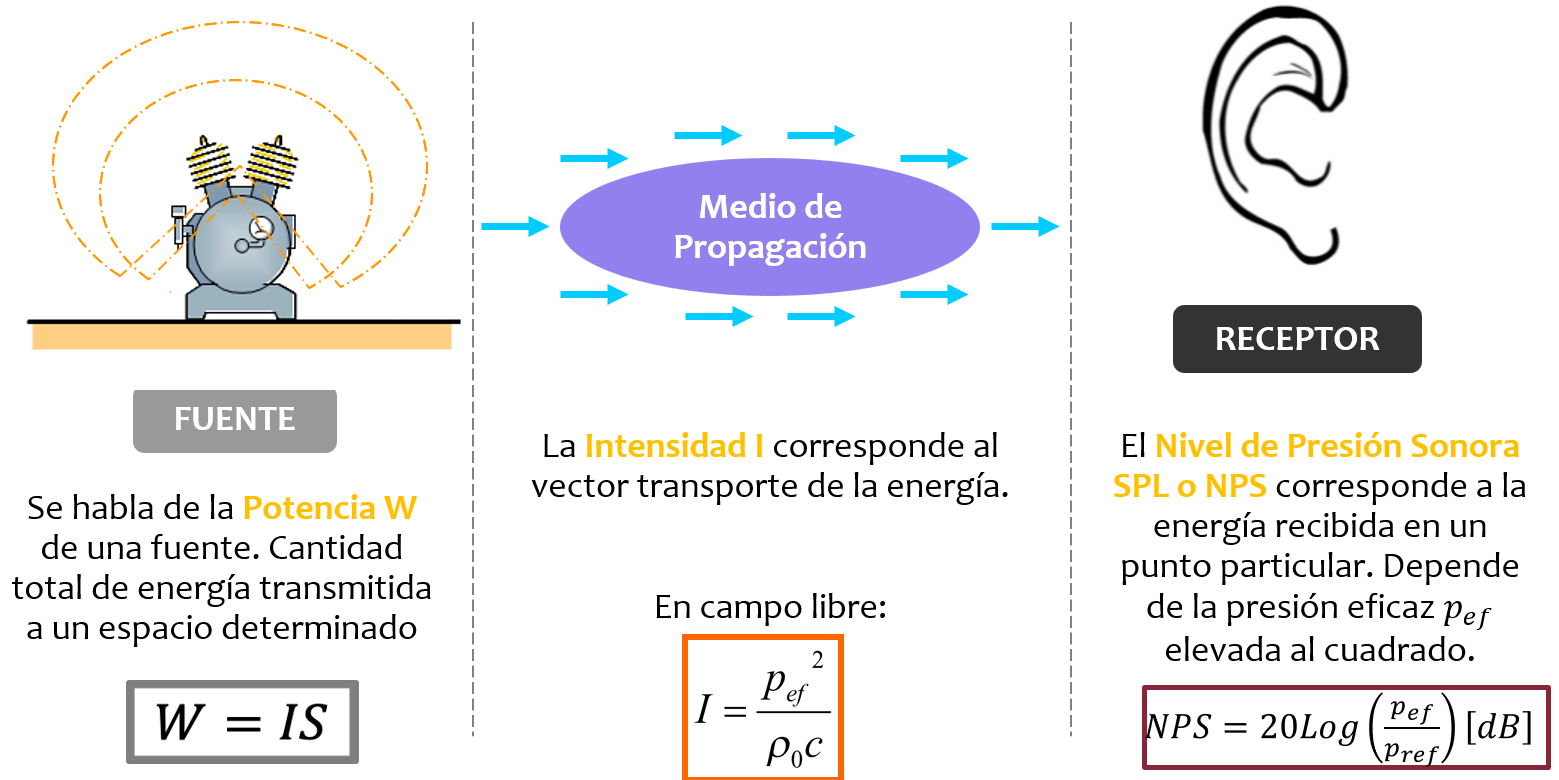
\includegraphics[width=1.0\textwidth]{figures/propagacion_sonido.png}
    \caption{Diagrama simple de una onda sonora viajando desde una fuente hasta el oído humano a través de un medio de propagación (imagen repetida de otro capítulo para afianzar el concepto).}
    \label{fig:propagacion-sonido-unidad-4}
\end{figure}

\section{Elasticidad y velocidad de propagación}
La velocidad del sonido ($c$) depende de la elasticidad ($E$, cómo el medio responde a la presión) y la densidad ($\rho$, cuánto pesan las partículas del medio):
\[
c = \sqrt{\frac{E}{\rho}}.
\]
En el aire, la velocidad aumenta con la temperatura:
\[
c \approx 331 + 0.6T \quad (\text{m/s, con } T \text{ en °C}).
\]
Por ejemplo, a 20°C, $c \approx 343$ m/s.

\begin{table}[h]
    \centering
    \begin{tabular}{|l|c|l|}
        \hline
        \textbf{Medio} & \textbf{Velocidad ($c$, m/s)} & \textbf{Observaciones} \\
        \hline
        Aire (20°C) & 343 & Condición estándar en audiometrías \\
        Agua (20°C) & 1480 & Usado en ultrasonidos médicos \\
        Hueso (aprox.) & 4000 & Relevante en audición ósea \\
        \hline
    \end{tabular}
    \caption{Velocidad del sonido en distintos medios.}
\end{table}

\begin{quote}
    \textbf{Ejemplo clínico.} En la audición ósea, el sonido viaja más rápido a través del cráneo (4000 m/s) que en el aire (343 m/s), lo que permite evaluar la cóclea directamente en pruebas audiométricas.
\end{quote}

\section{Propiedades de la onda acústica}
Las ondas sonoras tienen cuatro propiedades clave:
\begin{description}
    \item[\textbf{Frecuencia ($f$ [Hz]):}] Cuántos ciclos por segundo. Determina la \emph{altura} (grave o aguda). Por ejemplo, 250 Hz es grave (como un tambor), 4000 Hz es agudo (como una ``s'').
    \item[\textbf{Longitud de onda ($\lambda$ [m]):}] Distancia de un ciclo: $\lambda = c/f$. Una frecuencia alta tiene una longitud de onda corta.
    \item[\textbf{Amplitud ($A$ [Pa]):}] Intensidad de la variación de presión. Comúnmente esto es lo que se le dice ``volumen'' del sonido, pero en física el término preciso es ``intensidad sonora'' dado que volumen es la medida del espacio tridimensional que ocupa un cuerpo.
    \item[\textbf{Fase ($\varphi$, rad):}] Punto de inicio del ciclo. Afecta cómo se combinan las ondas.
\end{description}

\begin{quote}
    \textbf{Ejemplo clínico.} En una audiometría, se prueba la audición con tonos de diferentes frecuencias (125 Hz a 8000 Hz) para evaluar rangos graves y agudos, y con amplitudes variables para medir umbrales de audición.
\end{quote}

\section{Campo acústico}
El entorno afecta cómo percibimos el sonido:
\begin{itemize}
    \item \textbf{Campo libre:} Sin reflexiones, como en una cabina audiométrica ideal. El sonido llega directamente desde la fuente.
    \item \textbf{Campo reverberante:} Con ecos, como en una iglesia. Dificulta la claridad del habla.
    \item \textbf{Campo difuso:} Energía sonora uniforme, como en una sala ruidosa.
\end{itemize}
La \emph{distancia crítica} es el punto donde el sonido directo y los ecos tienen la misma intensidad. En cabinas audiométricas, se minimizan los ecos para garantizar mediciones precisas.

\begin{quote}
    \textbf{Ejemplo clínico.} Una cabina audiométrica usa paredes absorbentes para crear un campo libre, asegurando que el paciente escuche solo el tono puro del audiómetro.
\end{quote}

\section{Ondas esféricas y cilíndricas}
\begin{description}
    \item[\textbf{Ondas esféricas:}] Se expanden desde una fuente puntual (como un parlante) en todas direcciones. La intensidad cae 6 dB cada vez que se duplica la distancia (ley del cuadrado inverso).
    \item[\textbf{Ondas cilíndricas:}] Se propagan en un tubo o corredor (como el canal auditivo). La intensidad cae 3 dB por duplicar la distancia.
\end{description}

\begin{quote}
    \textbf{Ejemplo clínico.} En el canal auditivo, el sonido se propaga como una onda cilíndrica, lo que ayuda a amplificar frecuencias altas antes de llegar al tímpano.
\end{quote}

\begin{figure}[h]
    \centering
    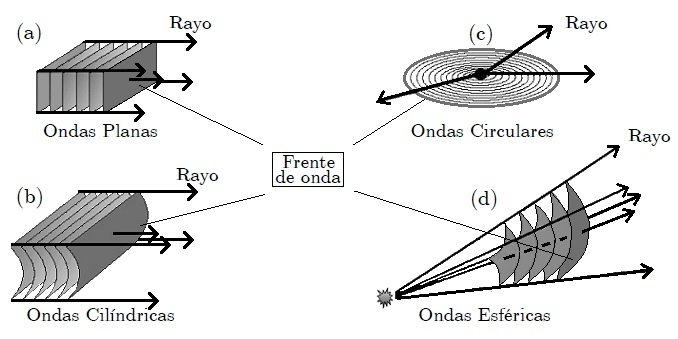
\includegraphics[width=1.0\textwidth]{figures/tipos_de_onda.jpg}
    \caption{Tipos de frente de onda.}
    \label{fig:tipos-de-onda}
\end{figure}


\section{Tono puro y señales complejas}
Un \textbf{tono puro} es un sonido con una sola frecuencia, como los tonos usados en audiometrías. Las \textbf{señales complejas} (como la voz o la música) son combinaciones de tonos puros (armónicos).

\begin{quote}
    \textbf{Ejemplo clínico.} La voz humana es una señal compleja con muchas frecuencias. En fonoaudiología, se analiza con herramientas como el espectrograma para detectar trastornos como la disfonía.
\end{quote}

\subsection{Valor RMS}
Para un tono puro, la presión RMS (raíz cuadrada media) mide la intensidad efectiva:
\[
P_{\text{RMS}} = \frac{P_0}{\sqrt{2}},
\]
donde $P_0$ es la amplitud pico. Esto se usa para calcular el nivel de presión sonora.


\begin{figure}[h]
    \centering
    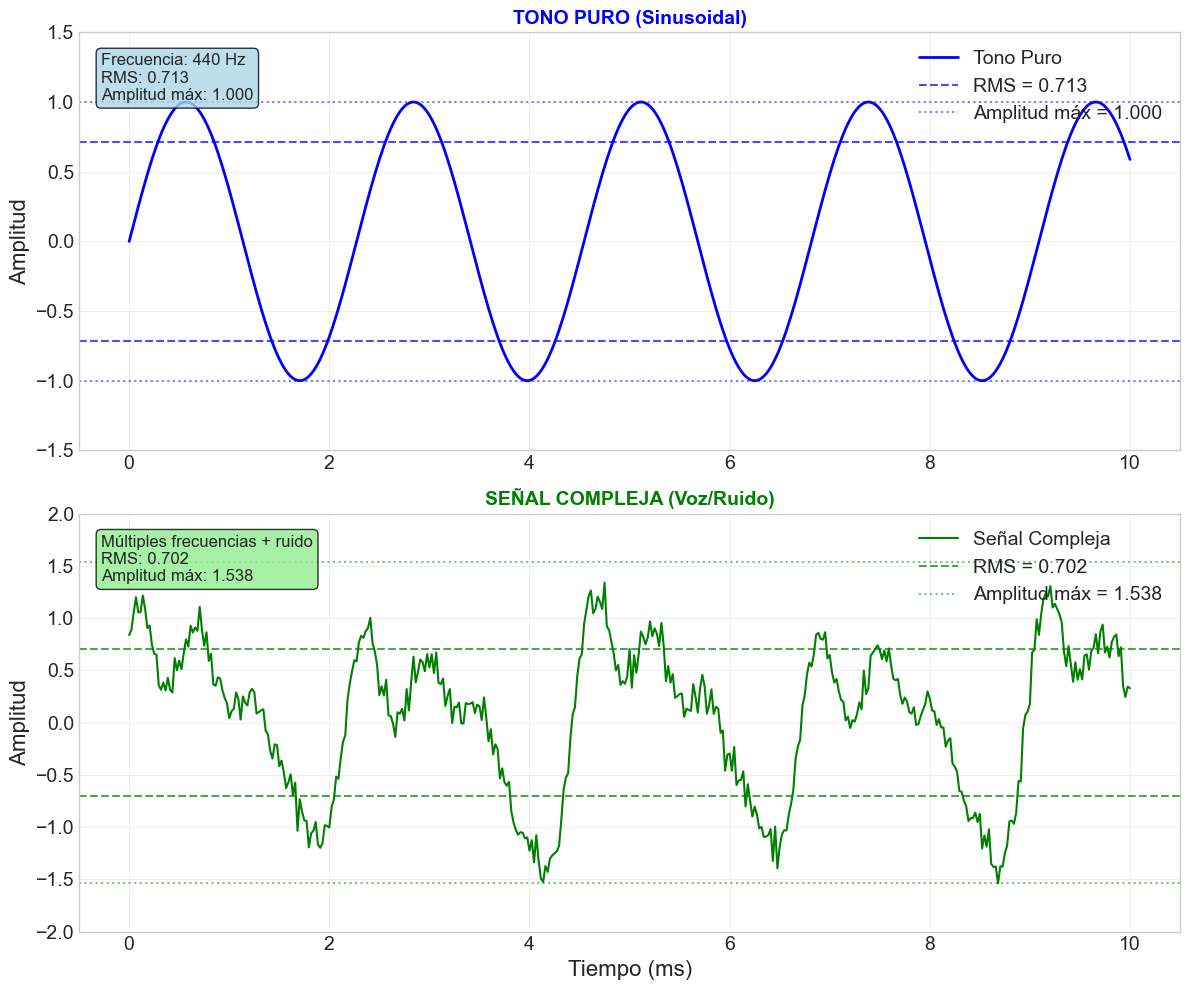
\includegraphics[width=1.0\textwidth]{figures/tono_vs_ruido.png}
    \caption{Comparación entre un tono puro y una señal compleja.}
    \label{tono_vs_ruido}
\end{figure}


\section{Presión sonora y nivel en decibeles}
El \textbf{nivel de presión sonora (SPL)} mide la intensidad del sonido en decibeles:
\[
L_p = 20 \log_{10}\left(\frac{P_{\text{RMS}}}{P_0}\right), \quad P_0 = 20~\mu\text{Pa}.
\]
La escala A (dBA) ajusta el nivel según la sensibilidad del oído humano, usada en audiometrías.

\begin{quote}
    \textbf{Ejemplo clínico.} Un tono de 60 dBA en una audiometría corresponde a una conversación normal, mientras que 20 dBA es un susurro.
\end{quote}

\section{Fuentes coherentes versus no coherentes}
\begin{description}
    \item[\textbf{Coherentes:}] Dos sonidos con la misma frecuencia y fase constante (como dos parlantes idénticos). Suman sus amplitudes, aumentando 6 dB si son iguales.
    \item[\textbf{No coherentes:}] Fases aleatorias (como dos personas hablando). Suman energías, aumentando 3 dB si los niveles son iguales.
\end{description}

\begin{figure}[h]
    \centering
    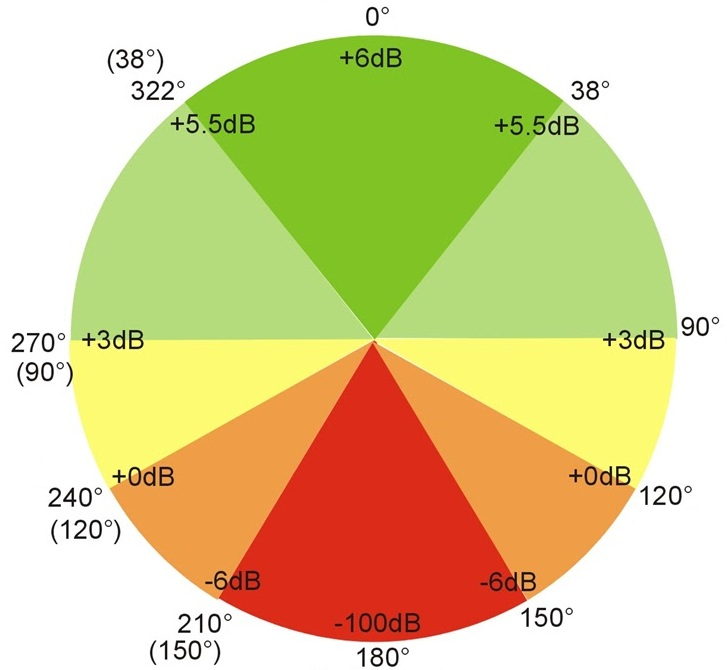
\includegraphics[width=0.6\textwidth]{figures/suma_fuentes.jpg}
    \caption{Resultado de suma de fuentes con diferente fase.}
    \label{suma_fuentes}
\end{figure}

\section{Ley del cuadrado inverso}
En un campo libre, la intensidad del sonido cae con la distancia:
\[
L_{p2} = L_{p1} - 20 \log_{10}\left(\frac{d_2}{d_1}\right).
\]
Por ejemplo, al duplicar la distancia (de 1 m a 2 m), el nivel cae 6 dB.

\begin{quote}
    \textbf{Ejemplo clínico.} Si un audiómetro produce 70 dB a 1 m en campo libre, a 2 m el nivel será 64 dB, lo que afecta la calibración en pruebas audiométricas.
\end{quote}


\section{Ejemplos prácticos}
\begin{enumerate}
    \item \textbf{Nivel a distancia.} Un altavoz omnidireccional produce 80 dB a 1 m. A 4 m:
    \[
    L_{p2} = 80 - 20 \log_{10}\left(\frac{4}{1}\right) \approx 80 - 12 = 68~\text{dB}.
    \]
    \item \textbf{Fuentes no coherentes.} Dos fuentes de 70 dB cada una suman:
    \[
    L_{\text{total}} = 10 \log_{10}(10^{70/10} + 10^{70/10}) \approx 73~\text{dB}.
    \]
    \item \textbf{Longitud de onda.} Para 500 Hz a 30°C ($c \approx 349$ m/s):
    \[
    \lambda = \frac{349}{500} \approx 0.7~\text{m}.
    \]
\end{enumerate}

\section{Ejercicios de autoevaluación}
\begin{enumerate}
    \item Explica por qué las frecuencias bajas (como un tambor) se escuchan mejor a larga distancia que las altas (como un silbido).
    \item Un audiómetro genera 70 dBSPL a 0.5 m. Calcula el nivel a 1.2 m en campo libre. (\emph{Solución}: $\approx 65.6$ dB.)
    \item En una cabina audiométrica, ¿por qué es importante minimizar las reflexiones para crear un campo libre?
\end{enumerate}

\section{Recursos recomendados}
\begin{itemize}
    \item Video: \href{https://www.youtube.com/watch?v=umTSWJ3POOk&ab_channel=AudioUniversity}{``INVERSE SQUARE LAW of Sound''}
    \item Libro: M. Raichel, \emph{Science and Applications of Acoustics}, capítulos 3–4.
    \item Libro: H. Fahy, \emph{Foundations of Engineering Acoustics}, sección 5.1.
\end{itemize}

\section*{Glosario}
\begin{description}
    \item[\textbf{Nivel de presión sonora (SPL):}] Intensidad del sonido en decibeles (dB).
    \item[\textbf{Directividad ($Q$):}] Cómo una fuente concentra el sonido en una dirección.
    \item[\textbf{Campo libre:}] Entorno sin reflexiones, ideal para audiometrías.
    \item[\textbf{Presión RMS:}] Valor efectivo de la presión sonora, usado en cálculos de dB.
    \item[\textbf{Onda longitudinal:}] Vibraciones en la dirección de propagación, como el sonido en el aire.
\end{description}

\section*{Resumen}
\begin{itemize}
    \item \textbf{Naturaleza del sonido:} Onda longitudinal que necesita fuente, medio y receptor.
    \item \textbf{Velocidad:} Depende de la elasticidad y densidad (343 m/s en aire, 4000 m/s en hueso).
    \item \textbf{Propiedades:} Frecuencia (altura), amplitud (sonoridad), fase (combinación).
    \item \textbf{Campo acústico:} Libre (sin ecos) o reverberante (con ecos), clave en cabinas.
    \item \textbf{Ley del cuadrado inverso:} La intensidad cae 6 dB al duplicar la distancia.
\end{itemize}


\bigskip
\noindent\emph{Conclusión.} Las propiedades del sonido (frecuencia, amplitud, fase) y las leyes de propagación (como la ley del cuadrado inverso) son esenciales para medir y entender la audición. Estos conceptos te ayudarán a calibrar audiómetros, diseñar entornos de prueba y analizar cómo el sonido llega al oído en diferentes condiciones. En la próxima unidad, exploraremos las herramientas para analizar y clasificar señales acústicas.


%%%%%%%%%%%%%%%%%%%%%%%%%%%%%%%%%%%%%%%%%%%%%%%%%%%%%%%%%%%%%%%%%%%%%%%%%%%%%%%%%%%%%%%%%%%%%%%%%%
